\section{最大化$\mathcal{l}(\theta)$的另一种算法}

回到逻辑回归问题,$g(z)$为sigmoid函数,让我们讨论另一种用于最大化$\mathcal{l}(\theta)$的算法。

让我们开始吧,考虑使用牛顿法寻找函数的零点。假设我们有一个函数$f:\mathbb{R}\rightarrow\mathbb{R}$,期望找到一个值$\theta$满足$f(\theta)=0$,其中$\theta \in \mathbb{R}$为实数。牛顿法进行如下操作:
$$
  \theta := \theta - \frac{f(\theta)}{f^\prime(\theta)}
$$
这个方法可以视为,在当前猜测值$\theta$处,通过一个正切于$f$的线性函数近似$f$,以求解该线性函数的零点,然后将下一个$\theta$设置为线性函数的零点。

\begin{figure}
  \begin{center}
    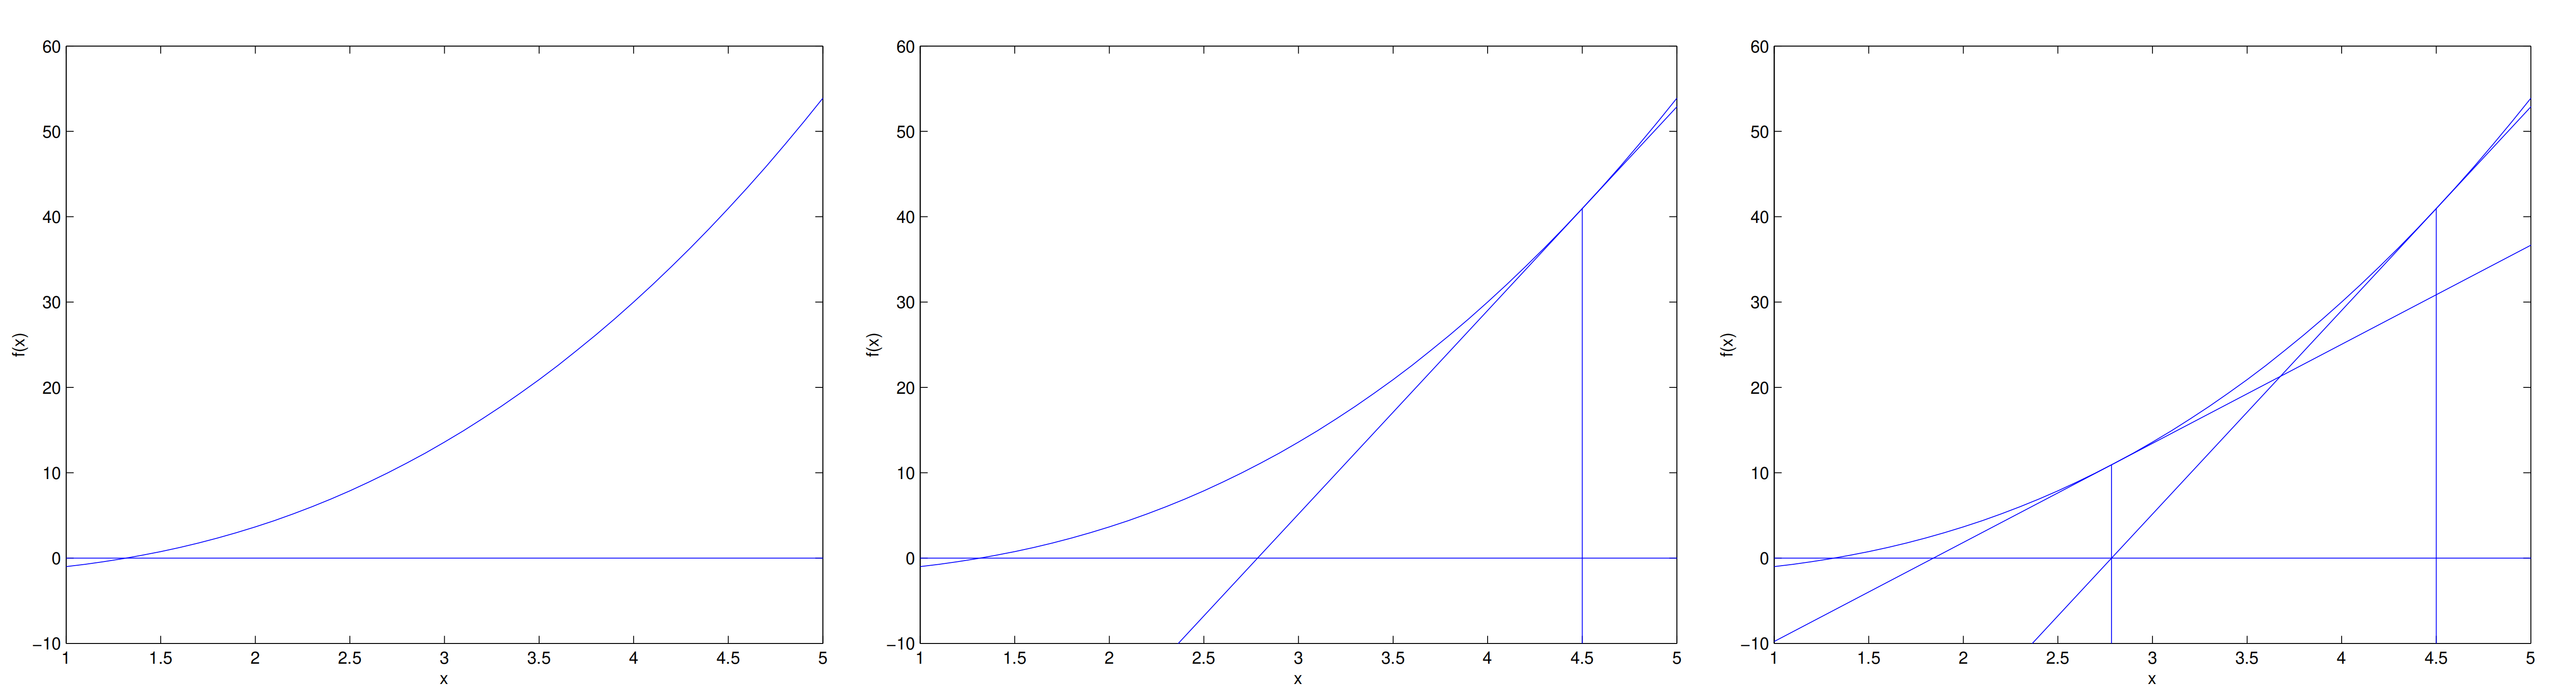
\includegraphics[width=0.9\textwidth]{imgs/2.4_newton.jpg}
  \end{center}
\end{figure}

这里有一张展示牛顿法具体步骤的图片:

在最左边的图片中,可以看到函数$f$与直线$y=0$绘制在一起,我们尝试寻找满足$f(\theta)=0$的$\theta$,能够满足这个目标的$\theta$约为$1.3$。假设我们设置$\theta$为$4.5$初始化此算法。
然后牛顿法在$\theta=4.5$处拟合一条正切于$f$的直线\footnote{译者注:此时直线为$y=f^{\prime}(4.5)x+f(4.5)-4.5f^{\prime}(4.5)$,零点$x=\frac{4.5f^{\prime}(4.5)-f(4.5)}{f^{\prime}(4.5)}=4.5-\frac{f(4.5)}{f^{\prime}(4.5)}$。},求解此直线的零点(中间的图片),并作为下一次迭代的猜测值,约为$2.8$,最右面的图片展示了下一次迭代的结果,将$\theta$更新为约$1.8$,再经过几次迭代后,我们将接近$\theta=1.3$。

牛顿法提供了寻找函数零点$f(\theta)=0$的方法,那么求解某个函数$\mathcal{l}$的最大值该如何处理呢?函数$\mathcal{l}$的最大值与一阶导数$\mathcal{l}^{\prime}(\theta)$的零点有关。因此,令$f(\theta)=\mathcal{l}^{\prime}(\theta)$,我们可以用同样的方法获取$\mathcal{l}$的极大值点,更新规则如下:
$$
\theta:=\theta-\frac{\mathcal{l}^{\prime}(\theta)}{\mathcal{l}^{\prime \prime}(\theta)}
$$
(思考题:如果我们想使用牛顿法寻找函数的最小值而不是最大值,需要做哪些调整?)

最后,在我们逻辑回归的定义中,$\theta$为向量值,因此我们需要推广牛顿法以满足这种定义,将牛顿法推广至多维定义的方法如下(也称为\textbf{Newton-Raphson}法):
$$
\theta:=\theta-H^{-1}\nabla_{\theta}\mathcal{l}(\theta)
$$
其中,$\nabla_{\theta}\mathcal{l}(\theta)$和通常一样,为$\mathcal{l}(\theta)$相对于$\theta_i$的偏导数向量,$H$为$d \times d$矩阵(实际上为$(d+1) \times (d+1)$,假设包括截距项),称为\textbf{Hessian},可以表示为:
$$
H_{ij}=\frac{\partial^2 \mathcal{l}(\theta)}{\partial \theta_i \partial \theta_j}
$$

相较于(批量)梯度下降,牛顿法的收敛速度更快,且通过较少的迭代即可非常接近最小值。但牛顿法的一次迭代相较于梯度下降复杂度更大,因为需要计算和求逆$d \times d$ Hession,但只要$d$不是很大,总体上还是快得多。当使用牛顿法最大化逻辑回归对数似然函数$\mathcal{l}(\theta)$时,这种方法称为\textbf{Fisher Scoring}。

